% !TeX spellcheck = en_US
\documentclass[./main.tex]{subfiles}
\begin{document}
	\subsection{Mobile app architecture}
	In this subsection, the decisions regarding the architecture of the mobile app will
	be explained, but not those that regard the user experience of the mobile. This 
	will be explained in more detail at  \ref{sec:views}.\\
	\\
	First, why we chose flutter and not other frameworks, as Android or React Native,
	will be explained. Then, it will be introduced the Redux for the state management
	of the app.\\
	\\
	\subsubsection{Flutter}
	Flutter is a multiplatform framework aiming to become a standard for building apps that have to work on either Android or iOS, as well as the web, desktop, and embedded operative systems. \\
	\\
	As a tool, it has been proven that it can build more resilient and optimized apps than its counterparts, like React Native, while still being multiplatform. Even though it was taught how to work with native Android Applications, it was decided to choose this tool against it as the team had already some experience with it.\\
	\\
	Even if the framework is young, the community behind flutter is active and has several repositories that have some application examples, as well as a libraries showcase that has and will help the development of the app.
	% TODO what the fuck did I just write?
	\subsubsection{Redux}
	State management in applications is a hot topic, and although both frameworks used by the clients in this project have some way to implement it, it was preferred to use a third-party option that is well consolidated, easy to use, and easy to manage.\\
	\\
	Redux is an abstraction that provides a way to implement easier a reactive pattern, that is, instead of having the typical Model-View-Controller, it has a way of drawing a State, the buttons can launch actions, that is taken by reducers along the actual state, and return the
	next state, as shown at \ref{fig:redux}.\\
	\\
	\begin{figure}[H]
		\centering
		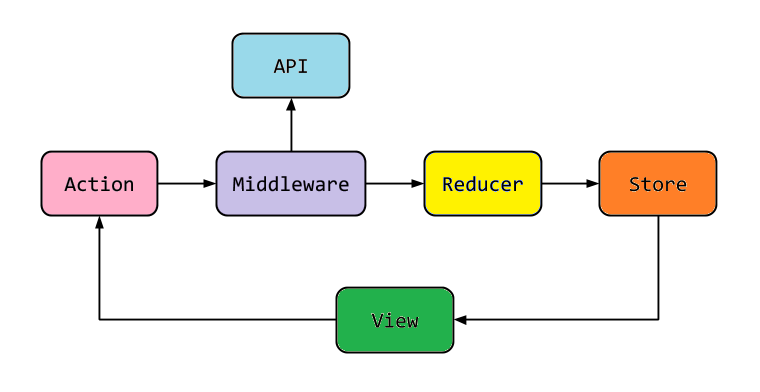
\includegraphics[width=0.8\textwidth]{img/redux.png}
		\caption{Redux Diagram.}
		\label{fig:redux}
	\end{figure}
	This makes the components stateless, which makes it easier to work with them and provides a way of mesmerizing them so they aren't computed that many times, making them faster than their counterparts. 
	\\
	\\
	This also helps to have a way of monitoring the changes that the state has suffered, as you can keep the states and the actions in a list for debugging, so it can be traced easily the changes. This adds when you have to have a shared object that won't be modified easily, but has to be read by most of the components, as an API token or a theme object.
	\\
	\\
	Finally, as it was also used in the web applications, it makes the team be able to change quickly between the two frameworks, as the most difficult part is done the same way.
	\\

	
\end{document}